\documentclass[12pt,a4paper]{article}

\usepackage[utf8]{inputenc}
\usepackage[T2A]{fontenc}
\usepackage[russian]{babel}
\usepackage{hyperref}
\usepackage[footnotes,oglav,spisok,boldsect,eqwhole,kursrab,remarks,hyperprint]{project}
\usepackage{graphicx}
\usepackage{float}
\graphicspath{{img/}}
\DeclareGraphicsExtensions{.pdf,.png,.jpg}

\begin{document}
%% FIRST DRAFT
\newpage
% \begin{multline}
%     \sum_{i=1}^{N} u_{i}\left[(\lambda+2 \mu) \dfrac{d \varphi_{i}}{d r}
%     \dfrac{d \varphi_{j}}{d r} \int \limits_{a}^{b} r d r+\lambda
%     \dfrac{d \varphi_{j}}{d r} \int\limits_{a}^{b} \varphi_{i} d r+\lambda
%     \dfrac{d \varphi_{i}}{d r} \int\limits_{a}^{b} \varphi_{j} d r+(\lambda+2 \mu)
%     \int\limits_{a}^{b} \dfrac{\varphi_{i} \cdot \varphi_{j}}{r} d r\right] = \\
%     = u_{i-1} \Bigg( (\lambda + 2\mu) \dfrac{d\varphi_i}{dr} \dfrac{d\varphi_{i-1}}{dr}
%     \int\limits_{r_{i-1}}^{r_i} r dr + \lambda \dfrac{d\varphi_{i-1}}{dr} \int\limits_{r_{i-1}}^{r_i} \varphi_i dr +
%     \lambda \dfrac{d\varphi_{i}}{dr} \int\limits_{r_{i-1}}^{r_i} \varphi_{i-1} dr +
%     (\lambda + 2\mu) \int\limits_{r_{i-1}}^{r_i} \dfrac{\varphi_i \cdot \varphi_{i-1}}{r}dr
%     \Bigg) + \\
%     + u_{i-1} \Bigg( 
%         (\lambda + 2\mu) \big(\dfrac{d\varphi_i}{dr}\big)^2
%         \int\limits_{r_{i-1}}^{r_i} r dr + (\lambda + 2\mu) \big(\dfrac{d\varphi_i}{dr}\big)^2
%         \int\limits_{r_{i}}^{r_{i + 1}} r dr + 2 \lambda \dfrac{d\varphi_i}{dr}
%         \int\limits_{r_{i-1}}^{r_i} \varphi_i dr + 2 \lambda \dfrac{d\varphi_i}{dr}
%         \int\limits_{r_{i}}^{r_{i+1}} \varphi_i dr + \\ + (\lambda + 2\mu)
%         \int\limits_{r_{i-1}}^{r_i} \dfrac{(\varphi_i)^2}{r}dr + (\lambda + 2\mu)
%         \int\limits_{r_{i}}^{r_{i + 1}} \dfrac{(\varphi_i)^2}{r}dr
%     \Bigg) + \\
%     + u_{i+1} \Bigg( (\lambda + 2\mu) \dfrac{d\varphi_i}{dr} \dfrac{d\varphi_{i+1}}{dr}
%     \int\limits_{r_{i}}^{r_{i+1}} r dr + \lambda \dfrac{d\varphi_{i+1}}{dr} \int\limits_{r_{i}}^{r_{i+1}} \varphi_i dr +
%     \lambda \dfrac{d\varphi_{i}}{dr} \int\limits_{r_{i}}^{r_{i+1}} \varphi_{i+1} dr +
%     (\lambda + 2\mu) \int\limits_{r_{i}}^{r_{i+1}} \dfrac{\varphi_i \cdot \varphi_{i+1}}{r}dr
%     \Bigg) = \\ = u_{i-1} a_i + u_i b_i + u_{i+1} c_i.
% \end{multline}

% $$
%     a_i = -(\lambda + 2\mu) \dfrac{r_i r_{i-1}}{h^2} \ln \dfrac{r_i}{r_{i-1}},
% $$

% $$
%     b_i = (\lambda + 2\mu) \big( \dfrac{r_{i-1}^2}{h^2} \ln \dfrac{r_i}{r_{i-1}} +
%     \dfrac{r_{i+1}^2}{h^2} \ln \dfrac{r_{i+1}}{r_{i}} \big),
% $$

% $$
%     c_i = -(\lambda + 2\mu) \dfrac{r_i r_{i+1}}{h^2} \ln \dfrac{r_i}{r_{i+1}},
% $$

% $$
% b_0 = (\lambda + 2\mu) \big(1 + \dfrac{r_{i+1}^2}{h^2}\ln \dfrac{r_{i+1}}{r_{i}}\big) + \lambda,
% \quad b_n = (\lambda + 2\mu) \big(-1 + \dfrac{r_{i-1}^2}{h^2}\ln \dfrac{r_{i}}{r_{i-1}}\big) + \lambda
% $$

% Система:
% $$
% \left\{\begin{array}{l}
%     u_0 b_0 + u_1 c_0 = \sigma_{rr}(a) r (a) = -p_a * a, \\
%     u_0 a_1 + u_1 b_1 + u_2 c_1 = 0, \\
%     \dots = \dots, \\
%     u_{n-2} a_{n-1} + u_{n-1} b_{n-1} + u_n c_{n-1} = 0, \\
%     u_{n-1} a_{n} + u_n b_n = \sigma_{rr}(b) r (b) = -p_b * b

% \end{array}\right.
% $$

%% SECOND DRAFT
% \newpage
% \begin{multline}
%     \sum_{i=1}^{N} u_{i}\left[(\lambda+2 \mu) \dfrac{d \varphi_{i}}{d r}
%     \dfrac{d \varphi_{j}}{d r} \int \limits_{a}^{b} r d r+\lambda
%     \dfrac{d \varphi_{j}}{d r} \int\limits_{a}^{b} \varphi_{i} d r+\lambda
%     \dfrac{d \varphi_{i}}{d r} \int\limits_{a}^{b} \varphi_{j} d r+(\lambda+2 \mu)
%     \int\limits_{a}^{b} \dfrac{\varphi_{i} \cdot \varphi_{j}}{r} d r\right] = \\
%     = u_{i-1} \Bigg( (\lambda + 2\mu) \dfrac{d\varphi_i}{dr} \dfrac{d\varphi_{i-1}}{dr}
%     \int\limits_{r_{i-1}}^{r_i} r dr + \lambda \dfrac{d\varphi_{i-1}}{dr} \int\limits_{r_{i-1}}^{r_i} \varphi_i dr +
%     \lambda \dfrac{d\varphi_{i}}{dr} \int\limits_{r_{i-1}}^{r_i} \varphi_{i-1} dr +
%     (\lambda + 2\mu) \int\limits_{r_{i-1}}^{r_i} \dfrac{\varphi_i \cdot \varphi_{i-1}}{r}dr
%     \Bigg) + \\
%     + u_{i-1} \Bigg( 
%         (\lambda + 2\mu) \big(\dfrac{d\varphi_i}{dr}\big)^2
%         \int\limits_{r_{i-1}}^{r_i} r dr + (\lambda + 2\mu) \big(\dfrac{d\varphi_i}{dr}\big)^2
%         \int\limits_{r_{i}}^{r_{i + 1}} r dr + 2 \lambda \dfrac{d\varphi_i}{dr}
%         \int\limits_{r_{i-1}}^{r_i} \varphi_i dr + 2 \lambda \dfrac{d\varphi_i}{dr}
%         \int\limits_{r_{i}}^{r_{i+1}} \varphi_i dr + \\ + (\lambda + 2\mu)
%         \int\limits_{r_{i-1}}^{r_i} \dfrac{(\varphi_i)^2}{r}dr + (\lambda + 2\mu)
%         \int\limits_{r_{i}}^{r_{i + 1}} \dfrac{(\varphi_i)^2}{r}dr
%     \Bigg) + \\
%     + u_{i+1} \Bigg( (\lambda + 2\mu) \dfrac{d\varphi_i}{dr} \dfrac{d\varphi_{i+1}}{dr}
%     \int\limits_{r_{i}}^{r_{i+1}} r dr + \lambda \dfrac{d\varphi_{i+1}}{dr} \int\limits_{r_{i}}^{r_{i+1}} \varphi_i dr +
%     \lambda \dfrac{d\varphi_{i}}{dr} \int\limits_{r_{i}}^{r_{i+1}} \varphi_{i+1} dr +
%     (\lambda + 2\mu) \int\limits_{r_{i}}^{r_{i+1}} \dfrac{\varphi_i \cdot \varphi_{i+1}}{r}dr
%     \Bigg) = \\ = u_{i-1} a_i + u_i b_i + u_{i+1} c_i.
% \end{multline}

% Вывод коэффициента $b$ для граничных узлов:

% \begin{equation}
%     \begin{gathered}
%     b_{0}=(\lambda+2 \mu)\left(\dfrac{d \varphi_{i}}{d r}\right)^{2} \int\limits_{r_{i}}^{r_{i+1}} r d r+(\lambda+2 \mu) \int\limits_{r_{i}}^{r_{i+1}} \dfrac{\left(d \varphi_{i}\right)^{2}}{r} d r+2 \lambda \dfrac{d \varphi_{i}}{d r} \int\limits_{r_{i}}^{r_{i+1}} \varphi_{i} d r= \\
%     =(\lambda+2 \mu)\left(\dfrac{1}{h^{2}} \dfrac{h\left(r_{i}+r_{i+1}\right)}{2}+\dfrac{r_{i}-3 r_{i+1}}{2 h}+\dfrac{r_{i+1}^{2}}{h^{2}} \ln \dfrac{r_{i+1}}{r_{i}}\right)+2 \lambda \dfrac{1}{h} \dfrac{h}{2}= \\
%     =(\lambda+2 \mu)\left(\dfrac{r_{i}+r_{i+1}+r_{i}-3 r_{i+1}}{2 h}+\dfrac{r_{i+1}^{2}}{h^{2}} \ln \dfrac{r_{i+1}}{r_{i}}\right) + \lambda= \\
%     =(\lambda+2 \mu)\left(\dfrac{r_{i}+r_{i} -h+r_{i}-3 r_{i} + 3h}{2 h}+\dfrac{r_{i+1}^{2}}{h^{2}} \ln \dfrac{r_{i+1}}{r_{i}}\right) + \lambda = \\
%     = (\lambda+2 \mu)\left(1+\dfrac{r_{i+1}^{2}}{h^{2}} \ln \dfrac{r_{i+1}}{r_{i}}\right) + \lambda
%     \end{gathered}
%     \end{equation}

% \begin{equation}
%     \begin{gathered}
%     b_{n}=(\lambda+2 \mu)\left(\dfrac{d \varphi_{i}}{d r}\right)^{2} \int\limits_{r_{i-1}}^{r_{i}} r d r+(\lambda+2 \mu) \int\limits_{r_{i-1}}^{r_{i}} \dfrac{\left(d \varphi_{i}\right)^{2}}{r} d r+2 \lambda \dfrac{d \varphi_{i}}{d r} \int\limits_{r_{i-1}}^{r_{i}} \varphi_{i} d r= \\
%     =(\lambda+2 \mu)\left(\dfrac{1}{h^{2}} \dfrac{h\left(r_{i}+r_{i-1}\right)}{2}+\dfrac{r_{i}-3 r_{i-1}}{2 h}+\dfrac{r_{i-1}^{2}}{h^{2}} \ln \dfrac{r_{i}}{r_{i-1}}\right)+2 \lambda \dfrac{1}{h} \dfrac{h}{2}= \\
%     =(\lambda+2 \mu)\left(\dfrac{r_{i}+r_{i-1}+r_{i}-3 r_{i-1}}{2 h}+\dfrac{r_{i-1}^{2}}{h^{2}} \ln \dfrac{r_{i}}{r_{i-1}}\right) + \lambda= \\
%     =(\lambda+2 \mu)\left(\dfrac{r_{i}+r_{i} + h +r_{i}-3 r_{i} -3h}{2 h}+\dfrac{r_{i-1}^{2}}{h^{2}} \ln \dfrac{r_{i}}{r_{i-1}}\right) + \lambda = \\
%     = (\lambda+2 \mu)\left(-1+\dfrac{r_{i-1}^{2}}{h^{2}} \ln \dfrac{r_{i}}{r_{i-1}}\right) + \lambda
%     \end{gathered}
% \end{equation}

% Система из двух узлов:
% $$
% \left\{\begin{array}{l}
%     u_0 b_0 + u_1 c_0 = \sigma_{rr}(a) r (a) = -p_a * a, \\
%     u_0 a_{1} + u_1 b_1 = \sigma_{rr}(b) r (b) = -p_b * b.
% \end{array}\right.
% $$

% $$
% \left\{\begin{array}{l}
%     u_0 \left( (\lambda+2 \mu)\left(1+\dfrac{r_{i+1}^{2}}{h^{2}} \ln \dfrac{r_{i+1}}{r_{i}}\right) + \lambda \right)
%     + u_1 \left(-(\lambda + 2\mu) \dfrac{r_i r_{i+1}}{h^2} \ln \dfrac{r_{i+1}}{r_{i}} \right)
%     = -p_a * a, \\
%     u_0 \left(-(\lambda + 2\mu) \dfrac{r_i r_{i-1}}{h^2} \ln \dfrac{r_i}{r_{i-1}} \right)
%     + u_1 \left( (\lambda+2 \mu)\left(-1+\dfrac{r_{i-1}^{2}}{h^{2}} \ln \dfrac{r_{i}}{r_{i-1}}\right) + \lambda \right)
%     = -p_b * b.
% \end{array}\right.
% $$

% $$
% \left\{\begin{array}{l}
%     u_0 \left( (\lambda+2 \mu)\left(1+\dfrac{b^{2}}{h^{2}} \ln \dfrac{b}{a}\right) + \lambda \right)
%     + u_1 \left(-(\lambda + 2\mu) \dfrac{a b}{h^2} \ln \dfrac{a}{b} \right)
%     = -p_a * a, \\
%     u_0 \left(-(\lambda + 2\mu) \dfrac{b a}{h^2} \ln \dfrac{b}{a} \right)
%     + u_1 \left( (\lambda+2 \mu)\left(-1+\dfrac{a^{2}}{h^{2}} \ln \dfrac{b}{a}\right) + \lambda \right)
%     = -p_b * b.
% \end{array}\right.
% $$
% Численные значения:
% \begin{equation*}
%     \left(
%     \begin{array}{cc}
%     4.7388 \cdot 10^{10} & -3.3141 \cdot 10^{10}\\
%     -3.3141 \cdot 10^{10} & 2.32557 \cdot 10^{10}
%     \end{array}
%     \right)
%     \left(
%         \begin{array}{c}
%         u_0\\
%         u_1
%         \end{array}
%     \right) =
%     \left(
%         \begin{array}{c}
%         0\\
%         -4 \cdot 10^{6}
%         \end{array}
%     \right)
%     \end{equation*}
% Решение:
% $$u_0 = -0.0356585, \quad  u_n = -0.0509878$$
% Параметры системы:

% $$
%     a = 0.03 \text{м}, \quad b = 0.04 \text{м},\quad p_a = 0 \text{Па},\quad
%     p_b = 10^8 \text{Па},\quad \nu = 0.25,\quad E = 2 \cdot 10^9  \text{Па}
% $$

%% Third DRAFT
% \newpage
% \begin{multline}
%         \sum_{i=1}^{N} u_{i}\left[(\lambda+2 \mu) \dfrac{d \varphi_{i}}{d r}
%         \dfrac{d \varphi_{j}}{d r} \int \limits_{a}^{b} r d r+\lambda
%         \dfrac{d \varphi_{j}}{d r} \int\limits_{a}^{b} \varphi_{i} d r+\lambda
%         \dfrac{d \varphi_{i}}{d r} \int\limits_{a}^{b} \varphi_{j} d r+(\lambda+2 \mu)
%         \int\limits_{a}^{b} \dfrac{\varphi_{i} \cdot \varphi_{j}}{r} d r\right].
% \end{multline}

% \begin{equation}
%     \begin{gathered}
%     b_{0}=(\lambda+2 \mu)\left(\dfrac{d \varphi_{i}}{d r}\right)^{2} \int\limits_{r_{i}}^{r_{i+1}} r d r+(\lambda+2 \mu) \int\limits_{r_{i}}^{r_{i+1}} \dfrac{\left(d \varphi_{i}\right)^{2}}{r} d r+2 \lambda \dfrac{d \varphi_{i}}{d r} \int\limits_{r_{i}}^{r_{i+1}} \varphi_{i} d r.
%     \end{gathered}
% \end{equation}

% \begin{equation}
%     \begin{gathered}
%     b_{n}=(\lambda+2 \mu)\left(\dfrac{d \varphi_{i}}{d r}\right)^{2} \int\limits_{r_{i-1}}^{r_{i}} r d r+(\lambda+2 \mu) \int\limits_{r_{i-1}}^{r_{i}} \dfrac{\left(d \varphi_{i}\right)^{2}}{r} d r+2 \lambda \dfrac{d \varphi_{i}}{d r} \int\limits_{r_{i-1}}^{r_{i}} \varphi_{i} d r.
%     \end{gathered}
% \end{equation}

% \begin{equation}
%     \begin{gathered}
%     a_i = (\lambda + 2\mu) \dfrac{d\varphi_i}{dr} \dfrac{d\varphi_{i-1}}{dr}
%         \int\limits_{r_{i-1}}^{r_i} r dr + \lambda \dfrac{d\varphi_{i-1}}{dr} \int\limits_{r_{i-1}}^{r_i} \varphi_i dr +
%         \lambda \dfrac{d\varphi_{i}}{dr} \int\limits_{r_{i-1}}^{r_i} \varphi_{i-1} dr +
%         (\lambda + 2\mu) \int\limits_{r_{i-1}}^{r_i} \dfrac{\varphi_i \cdot \varphi_{i-1}}{r}dr
%     \end{gathered}
% \end{equation}

% \begin{equation}
%     \begin{gathered}
%     c_i = (\lambda + 2\mu) \dfrac{d\varphi_i}{dr} \dfrac{d\varphi_{i+1}}{dr}
%         \int\limits_{r_{i}}^{r_{i+1}} r dr + \lambda \dfrac{d\varphi_{i+1}}{dr} \int\limits_{r_{i}}^{r_{i+1}} \varphi_i dr +
%         \lambda \dfrac{d\varphi_{i}}{dr} \int\limits_{r_{i}}^{r_{i+1}} \varphi_{i+1} dr +
%         (\lambda + 2\mu) \int\limits_{r_{i}}^{r_{i+1}} \dfrac{\varphi_i \cdot \varphi_{i+1}}{r}dr
%     \end{gathered}
% \end{equation}

%% Fourth draft
% \newpage
% $$
% \left\{\begin{array}{l}
%     u_0 b_0 + u_1 c_0 = \sigma_{rr}(a) r (a) = 0, \\
%     u_0 a_{1} + u_1 b_1 = \sigma_{rr}(b) r (b) = -P_b b.
% \end{array}\right.
% $$
% Параметры системы:
% $$
%     a = 0.03 \text{м}, \quad b = 0.04 \text{м},\quad p_a = 0 \text{Па},\quad
%     p_b = 10^6 \text{Па},\quad \nu = 0.3,\quad E = 2 \cdot 10^{11}  \text{Па}
% $$
% Коэффициент $b_0$ (я его немного преобразовал):
% $$
%     b_0 = \frac{b^2 (\lambda+2 \mu) \ln \left(\frac{b}{a}\right)}{(a-b)^2}-2 (\lambda+ \mu)
% $$
% Аналитическое решение:
% $$
% u=\frac{1-2 \nu}{E} \frac{p_{a} a^{2}-p_{b} b^{2}}{b^{2}-a^{2}}
% r+\frac{1+\nu}{E} \frac{a^{2} b^{2}}{r} \frac{p_{a}-p_{b}}{b^{2}-a^{2}} .
% $$
% Пусть задано граничное условие первого рода в т. $b$:
% $$
%     u(b) = u(0.04) = -6.54286 \cdot 10^{-6}
% $$
% Тогда
% $$
% \begin{array}{l}
%     u_0 b_0 + u_1 c_0 = 0;\\
%     u_0 = -\dfrac{u_1 c_0}{b_0}
% \end{array}
% $$

% \begin{equation}
%     \begin{gathered}
%     c_i = (\lambda + 2\mu) \dfrac{d\varphi_i}{dr} \dfrac{d\varphi_{i+1}}{dr}
%         \int\limits_{r_{i}}^{r_{i+1}} r dr + \lambda \dfrac{d\varphi_{i+1}}{dr} \int\limits_{r_{i}}^{r_{i+1}} \varphi_i dr +
%         \lambda \dfrac{d\varphi_{i}}{dr} \int\limits_{r_{i}}^{r_{i+1}} \varphi_{i+1} dr +
%         (\lambda + 2\mu) \int\limits_{r_{i}}^{r_{i+1}} \dfrac{\varphi_i \cdot \varphi_{i+1}}{r}dr
%     \end{gathered}
% \end{equation}

% \begin{figure}[h]
%     \center{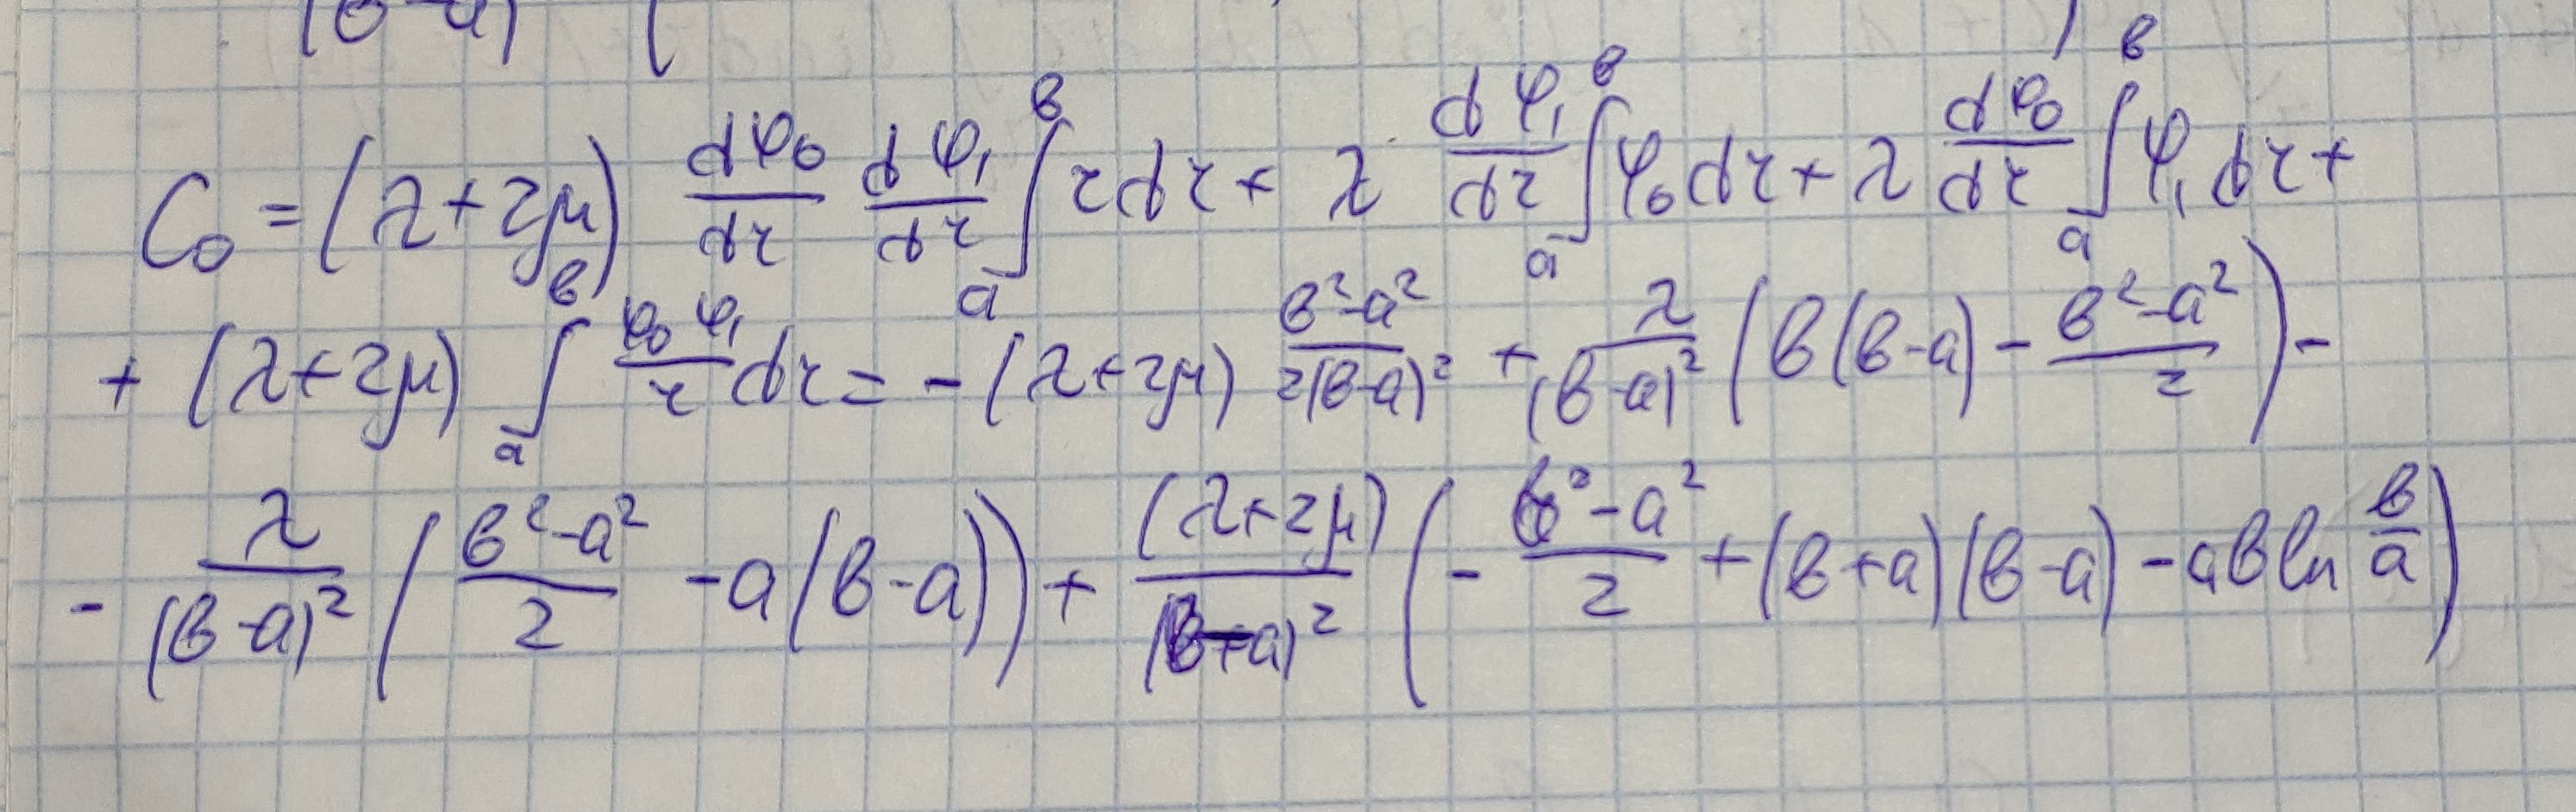
\includegraphics[scale=0.15]{1.jpg}}
%     \label{fig:image}
% \end{figure}
% $c_0 = -9.42045 \cdot 10^{11}$.
% Приблительное значение $u_0$:
% $$u_0 = -7.21208 \cdot 10^{-6}$$
% Точное значение $u_0$:
% $$u_0 = -6.85714 \cdot 10^{-6}$$

% \textit{Аналогично для второго уравнения}:
% $$
% \begin{array}{l}
%     u_0 a_1 + u_1 b_1 = -P_b b;\\
%     u_1 = \dfrac{ -P_b b - a_1 u_0}{b_1}
% \end{array}
% $$

% \begin{equation}
%     \begin{gathered}
%     a_i = (\lambda + 2\mu) \dfrac{d\varphi_i}{dr} \dfrac{d\varphi_{i-1}}{dr}
%         \int\limits_{r_{i-1}}^{r_i} r dr + \lambda \dfrac{d\varphi_{i-1}}{dr} \int\limits_{r_{i-1}}^{r_i} \varphi_i dr +
%         \lambda \dfrac{d\varphi_{i}}{dr} \int\limits_{r_{i-1}}^{r_i} \varphi_{i-1} dr +
%         (\lambda + 2\mu) \int\limits_{r_{i-1}}^{r_i} \dfrac{\varphi_i \cdot \varphi_{i-1}}{r}dr
%     \end{gathered}
% \end{equation}

% \begin{figure}[h]
%     \center{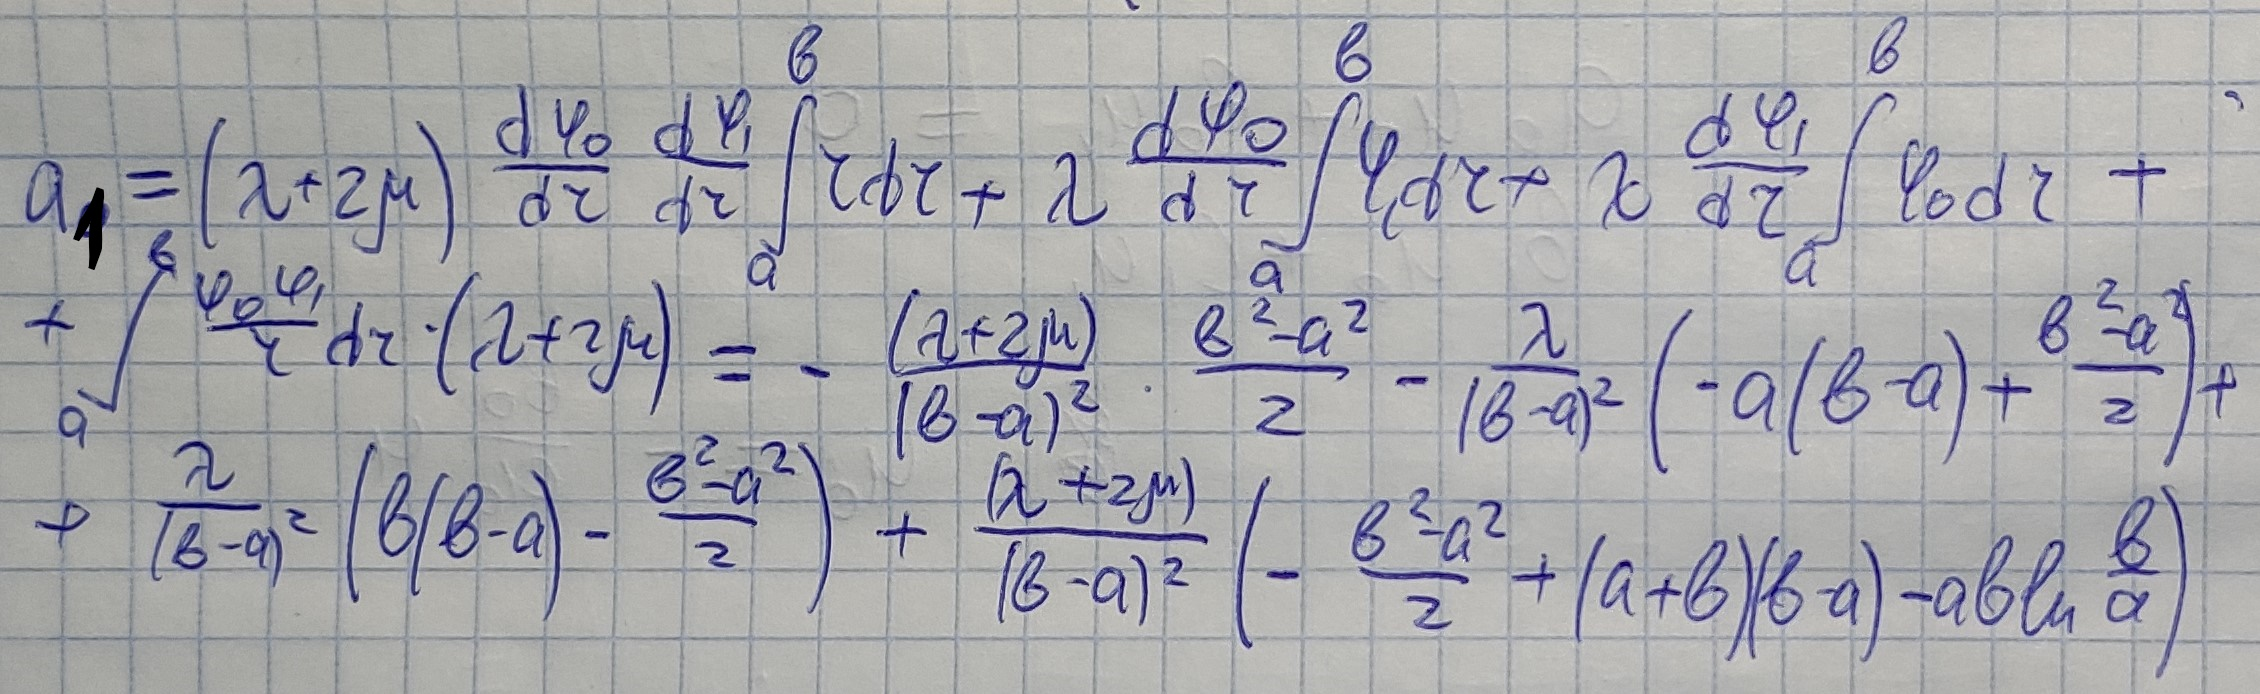
\includegraphics[scale=0.20]{a11.jpg}}
%     \label{fig:image}
% \end{figure}
% Численное значение:
% $$a_1 = -9.42045 \cdot 10^{11}$$

% Коэффициент $b_1$:
% \begin{figure}[h]
%     \center{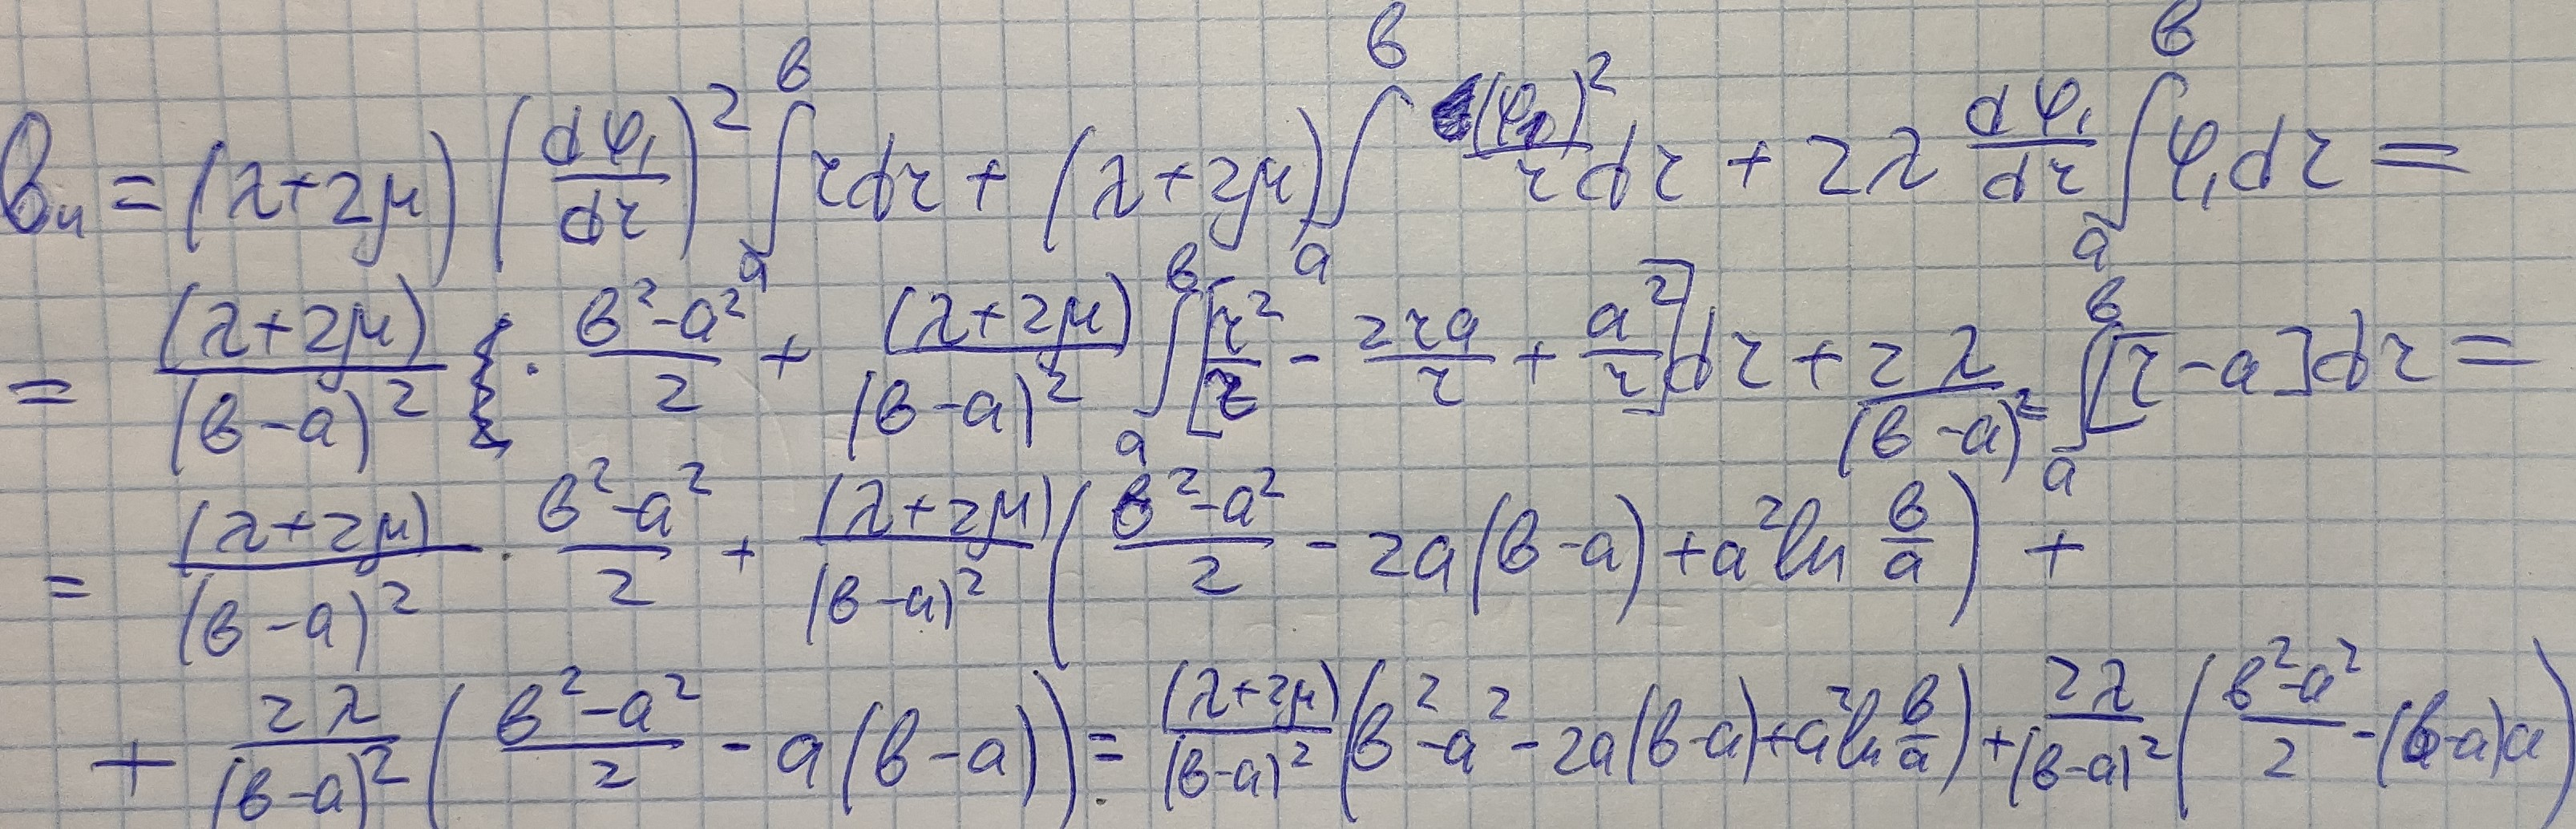
\includegraphics[scale=0.20]{bn.jpg}}
%     \label{fig:image}
% \end{figure}

% Численное значение:
% $$b_1 = 1.08169 \cdot 10^{12}$$

% Тогда численное значение $u_1$:
% $$
% u_1 = \dfrac{ -P_b b - a_1 u_0}{b_1} = -6.34168\cdot 10^{-6}
% $$
% Точное:
% $$
% u_1 = -6.54286\cdot 10^{-6}
% $$

% Fifth
Параметры системы:
$$
    a = 0.03 \text{м}, \quad b = 0.04 \text{м},\quad p_a = 0 \text{Па},\quad
    p_b = 10^6 \text{Па},\quad \nu = 0.3,\quad E = 2 \cdot 10^{11}  \text{Па}
$$
Аналитическое решения из Феодосьева:
\begin{figure}[H]
    \center{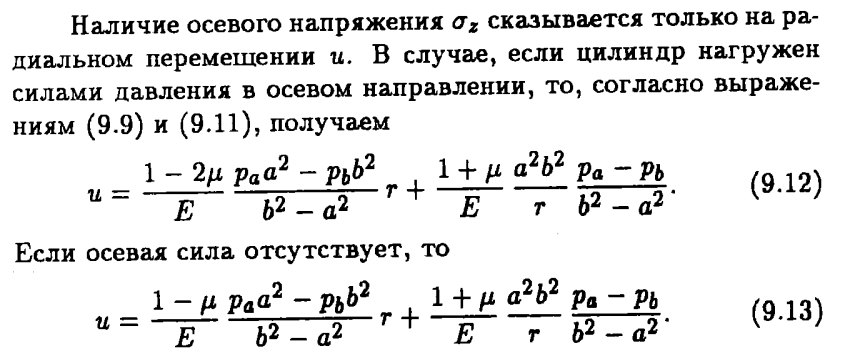
\includegraphics[scale=0.5]{Resh.png}}
    \label{fig:image}
\end{figure}
Аналитическое решение (9.12) и приближенное:
\begin{figure}[H]
    \center{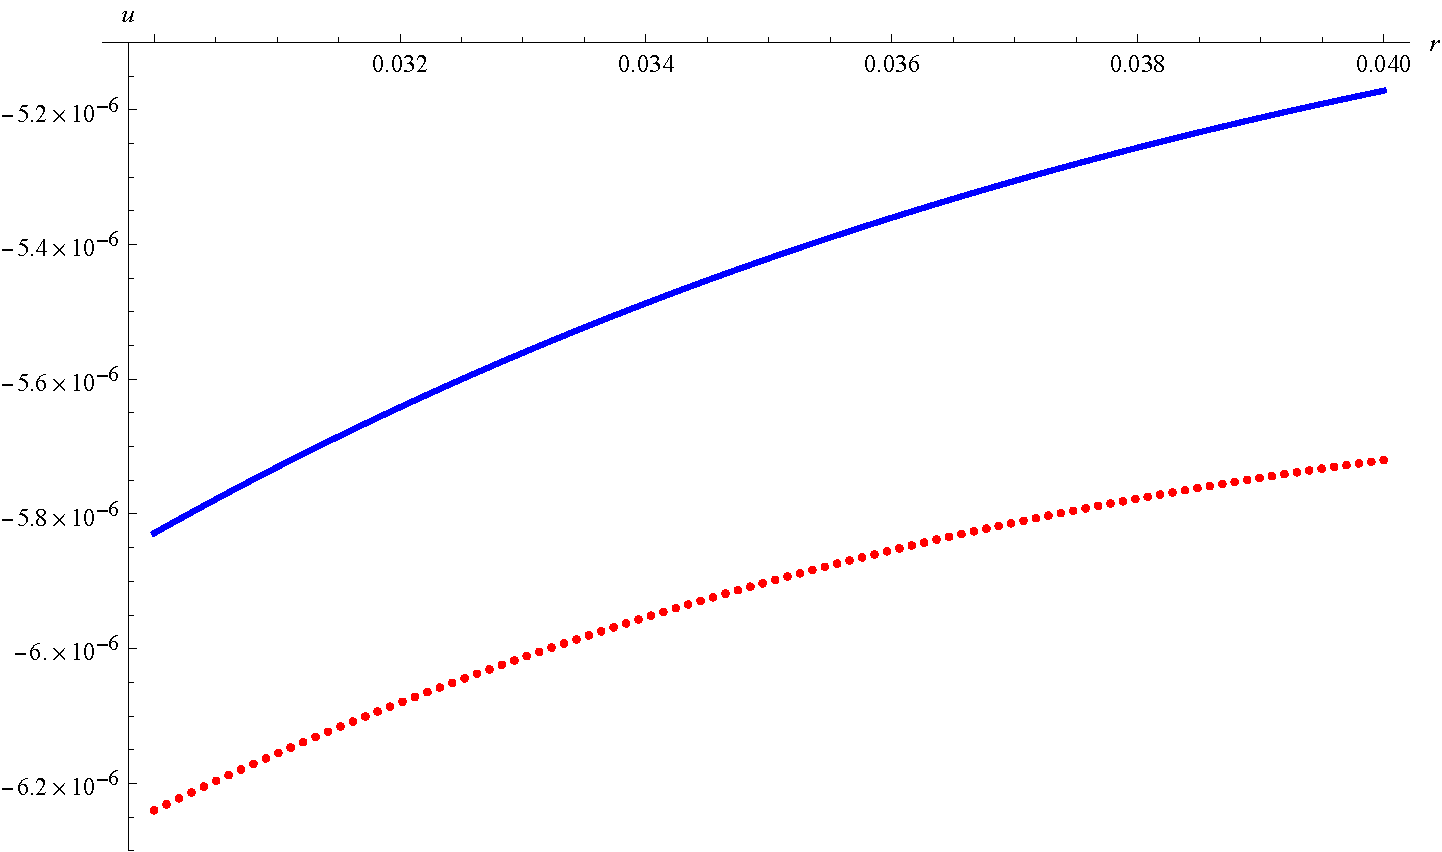
\includegraphics[scale=0.7]{1.pdf}}
    \label{fig:image}
\end{figure}
Система при 10 узлах:
\begin{figure}[H]
    \center{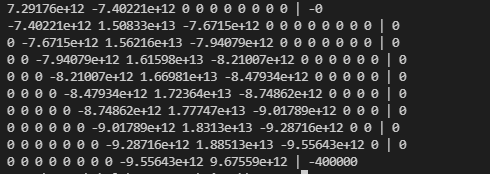
\includegraphics[scale=1]{Sist.png}}
    \label{fig:image}
\end{figure}
\end{document} 